

\documentclass{article}
\usepackage{graphicx}

\title{Dependable Distributed Systems}
\author{Ashkan Ansarifard}
\date{Start date: February 11, 2023 \\ Last modified: \today}

\begin{document}
	
\maketitle
\newpage
\tableofcontents
	
\newpage
\newpage
\section{Modelling Distributed Systems}
A distributed system is a set of entities, computes or machines communicating, coordinating and sharing resources to reach a common goal, appearing as a single computing system.

\newpage
\section{Time in Distributed Systems}

\newpage
\section{Logical Clock}

\newpage
\section{Distributed Mutual Exclusion}

\newpage
\section{Failure Detection Abstraction}
A \textbf{failure detector abstraction} is a software module used to detect faulty processes, it encapsulate timing assumptions of a either partially synchronous or fully synchronous system. It has two properties:
\begin{itemize}
	\item \textbf{Accuracy}: that represents the ability to avoid mistakes
	\item \textbf{Completeness}: that represents the ability to detect all failures
\end{itemize}

\subsection{Perfect Failure Detectors}
\label{sec:perfect-failure-detectors}
Here is a figure that illustrates the specifications of perfect failure detectors:
\begin{figure}[h]
	\centering
	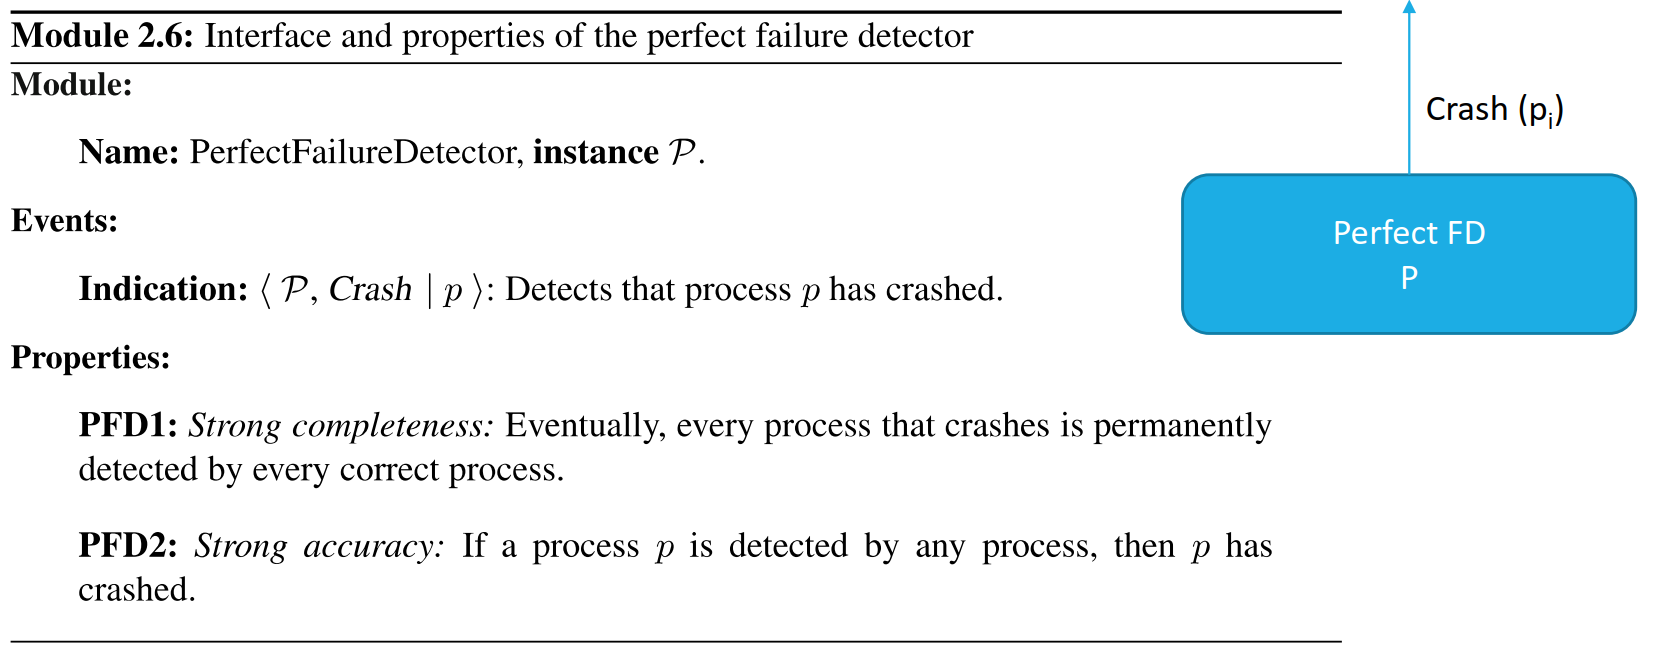
\includegraphics[width=0.9\linewidth]{resources/images/chapter 5/Perfect_Failure_Detector_Specifications.png}
	\caption{Specifications of perfect failure detectors}
	\label{fig:perfect-failure-detector-specifications}
\end{figure}

\subsection{Eventually Perfect Failure Detectors}

\subsection{Leader Election}

\subsection{Eventual Leader Election}

\newpage
\section{Broadcast Communications}

\newpage
\section{Consensus}

\newpage
\section{Ordered Communications}

\newpage
\section{Registers}

\newpage
\section{Software Replication}

\newpage
\section{Overview on Capacity Planning}

\newpage
\section{Modeling the Workload of a System}

\newpage
\section{Building a Performance Model 1}

\newpage
\section{Building a Performance Model 2}

\newpage
\section{Dependability Evaluation}

\newpage
\section{Intro to Experimental Design}

\newpage
\section{CAP Theorem}

\newpage
\section{Consistency Criteria for Distributed Shared Memories}

\newpage
\section{Publish-Subscribe Communication Paradigm}

\newpage
\section{Overlay Networks}

\newpage
\section{DLT and Blockchain}
	
\newpage
\section{Exercises}
\emph{Notice: The exercises are from 2022-2023 academic year.}

\newpage
\section{Exams}

	
\end{document}\dfrac{num}{den}